\chapter{Desenvolvemento da Unidade Didáctica}\label{chap:desenvolvemento}
Durante este capítulo describiremos o corpo do traballo, é decir, o deseño da unidade didáctica. Empezaremos detallando o contexto sobre o que se basea esta unidade, a continuación durante dúas secións detalleremos os elementos que a forman e as súas características e por último faremos unha valoración da aplicación dalgunhas das partes deste traballo durante as prácticas curriculares que se realizaron como parte do mestrado.

Para a descripción dos contidos e características da unidade didáctica seguiremos en parte o esquema proposto por Del~Valle~(2004 en \citeNP{delvalleud}). A autora propón que debe estar formada por unha parte de \textbf{descripción}, onde se detalle o nome da unidade, curso ao que vai dirixido, temporalizacion e a relación cos obxectivos de etapa; e outra parte de \textbf{elementos} na que se tratan os contidos, a metodoloxía empregada, a avaliación, os recursos empregados, a atención a diversidade, os temas transversais, así como a proposta de actividades. A este esquema engadiremos unha fundamentación temática e unha xustificación curricular na parte de descripción así como dedicar especial atención aos estandares de aprendizaxe avaliables por ser esta unha das partes máis subliñables pola actual lexislación.

\section{Contextualización da Unidade Didáctica}
É importante coñecer o contexto no que está baseado esta unidade didáctica. Isto é a características do centro e a clase nas que se vai impartir.

Esta unidade didáctica está orientada para os alumnos dunha clase de \textbf{1º de ESO} do \textbf{IES.~Leiras~Pulpeiro} de Lugo. Trátase dun centro público de ensino secundario creado no ano 1998 nun dos barrios periféricos de Lugo. Na actualidade impártense nel clases de Ensino Secundario Obrigatorio, Bacharelato e Ciclo Formativo de Grao Superior de Industrias Alimentarias e conta con moi boa fama dentro dos institutos da cidade.

En canto as características socio-económicas da poboación do centro, como aparece no Proxecto Educativo de Centro, ``pola súa situación, unha zona periférica con poboación asentada en vivendas sociais, defínese unha estrutura socio-económica media-baixa''. O alumnado que acolle é variado, a súa poboación está formada por unha parte de nenos e nenas do barrio, con presenza da etnia xitana; outra parte da contorna rural, alumando inmigrante, con procedencia latinoamericana sobre todo; e en menor cantidade outro conxunto de alumnos que por motivos disciplinarios chega doutros centros.

En canto a estrutura física e a situación do instituto, este atópase situado nunha parcela de $8000 m^2$ dos cales está construídos uns $6600 m^2$. O espazo co que conta o instituto cobre ben as súas necesidades posibilitando incluso a formación de grupos reducidos para os alumnos con dificultades. As aulas están organizadas do xeito tradicional, se ben existen elementos na aula que pretenden certa innovación como a disposición de unha biblioteca de aula, un corcho onde os alumnos pegan os seus traballos e equipamento informático como ordenadores tanto para o profesor como para o alumnado (proxecto Abalar\footnote{\href{https://www.edu.xunta.es/espazoAbalar/espazo/proxecto-abalar/introducion}{edu.xunta.es/espazoAbalar/espazo/proxecto-abalar/introducion}}), proxector e encerado dixitais na maior parte de aulas.

%TODO: description alumnos.

\section{Descripción da Unidade Didáctica}
A unidade didáctica deseñada titúlase ``Figuras xeométricas planas. Concepto e propiedades'' e está dirixida a alumnos e alumnad de 1º de ESO. De seguido explicaremos porque se elexíu este tema e a súa localización dentro da normativa vixente e temporalmente dentro do curso académico.

\subsection{Fundamentación temática}
%• Fundamentación mediante a achega relevante e actualizada de documentos que versaren sobre a temática elixida e sustentada en achegas de investigación didáctica.

\subsection{Xustificación da unidade}
%• Xustificación da unidade atendendo á lexislación vixente (decretos, reais decretos de ensinanzas mínimas, e ordes), a outros aspectos psicopedagóxicos e didácticos que xustificaren a súa inclusión no currículo da etapa, e/ou o curso e a súa contextualización.

\subsection{Temporalización}
Esta unidadade didáctica dura un total de


\section{Elementos da unidade didáctica}
% Elementos da unidade didáctica claramente diferenciados e efinidos: expectativas de aprendizaxe (obxectivos e competencias básicas), contidos, temporalización, metodoloxía e recursos.
Nesta sección explicaremos a forma na que esta unidade pretende acadar os obxectivos de etapa e os estandares de aprendizaxe qeu prentendemos lograr con ela, a forma en que contribue ao logro das competencias clave, os contidos que pretendemos que adquiran os alumnos, a meteodoloxía desenvolvida, os recursos empregados, as medidas de atención a diversidade, os ferramentas empregadas para avaliar ao alumnado e, por último, as actividades propostas.

\subsection{Obxectivos de etapa e estándares de aprendizaxe}
%Obxectivos e competencias básicas.

En \cite{dogcurrlomce} vemos que se definen obxectivos como ``referentes relativos aos logros que o alumnado debe alcanzar ao rematar o proceso educativo, como resultado das experiencias de ensino e aprendizaxe intencionalmente planificadas para tal fin''. Neste decreto tamén se establecen os obxectivos para a etapa de educación secundaria. A continucación veremos como esta unidade pretende axudar a consecución dalgún destos obxectivos de etapa.

A través do traballo en equipos heteroxéneos no que se intentará mesturar alumnado de diferente sexo, etnia, nacionalidade e nivel de rendemento académico intentaremos traballar os seguintes obxectivos de etapa:

\begin{itemize}
    \item Asumir responsablemente os seus deberes, coñecer e exercer os seus dereitos no respecto ás demais persoas, practicar a tolerancia, a cooperación e a solidariedade entre as persoas e os grupos, exercitarse no diálogo, afianzando os dereitos humanos e a igualdade de trato e de oportunidades entre mulleres e homes, como valores comúns dunha sociedade plural, e prepararse para o exercicio da cidadanía democrática.

    \item Desenvolver e consolidar hábitos de disciplina, es e iniciarse no coñecemento, na lectura e no estudo da literatura.tudo e traballo individual e en equipo, como condición necesaria para unha realización eficaz das tarefas da aprendizaxe e como medio de desenvolvemento persoal.

    \item Valorar e respectar a diferenza de sexos e a igualdade de dereitos e oportunidades entre eles. Rexeitar a discriminación das persoas por razón de sexo ou por calquera outra condición ou circunstancia persoal ou social. Rexeitar os estereotipos que supoñan discriminación entre homes e mulleres, así como calquera manifestación de violencia contra a muller.

    \item Rexeitar a violencia, os prexuízos de calquera tipo e os comportamentos sexistas, e resolver pacificamente os conflitos durante os traballos en equipo.
\end{itemize}

A través da exposición do traballo feito en equipo pretendemos que o alumnado consiga o obxectivo:

\begin{itemize}
    \item Comprender e expresar con corrección, oralmente e por escrito, na lingua galega e na lingua castelá, textos e mensaxes complexas.
\end{itemize}

Realizando actividades nas que se lle pide á toda a clase que presenten como resolverían un determinado problema expoñendo as razóns polas que creen que a súa resposta é a correcta intentamos que o alumnado logre o obxectivo de etapa:
\begin{itemize}
    \item Desenvolver o espírito emprendedor e a confianza en si mesmo, a participación, o sentido crítico, a iniciativa persoal e a capacidade para aprender a aprender, planificar, tomar decisións e asumir responsabilidades.
\end{itemize}

Realizando actividades onde se lle pide aos alumnos e alumnas que procuren definicións en internet traballamos o obxectivo:
\begin{itemize}
    \item Desenvolver destrezas básicas na utilización das fontes de información, para adquirir novos coñecementos con sentido crítico. Adquirir unha preparación básica no campo das tecnoloxías, especialmente as da información e a comunicación.
\end{itemize}

Creando actividades nas que os alumnos se informan da historia de certo concepto matemático fomentamos un maior logro do obxectivo:

\begin{itemize}
    \item Coñecer, valorar e respectar os aspectos básicos da cultura e da historia propias e das outras persoas, así como o patrimonio artístico e cultural.
\end{itemize}

Empregando o galego como lingua vehicular na clase intentase traballar o obxectivo:

\begin{itemize}
    \item Coñecer e valorar a importancia do uso da lingua galega como elemento fundamental para o mantemento da identidade de Galicia.
\end{itemize}

Da mesma forma, en \cite{dogcurrlomce} defínense os estándares de aprendizaxe como ``especificacións dos criterios de avaliación que permiten definir os resultados de aprendizaxe e que concretan o que o alumnado debe saber, comprender e saber facer en cada disciplina.''.  Os estándares de aprendizaxe para esta unidade didáctica son os seguintes:

\begin{enumerate}[label=\bfseries Est\arabic*]
 \item\label{est1} Recoñece e describe elementos de xeometría tales como o punto, a recta ou o ángulo.
 \item\label{est2} Clasifica rectas e ángulos en función da súa posición relativa.
 \item\label{est3} Clasifica ángulos en función da súa amplitude.
 \item\label{est4} Emprega o sistema sesaxesimal para o cálculo de sumas e restas de ángulos.
 \item\label{est5} Define as características de mediatriz e bisectriz e sabe trazalas.
 \item\label{est6} Identifica elementos dos polígonos.
 \item\label{est7} Clasifica polígonos en función do número de lados e os seus ángulos.
 \item\label{est8} Clasifica triángulos e cuadriláteros en función das súas propiedades.
 \item\label{est9} Define os puntos e rectas notables dun triángulo e sabe trazalas.
 \item\label{est10} Resolve problemas de xeometría empregando o teorema de Pitágoras.
 \item\label{est11} Explica as propiedades dos puntos dunha circunferencia.
 \item\label{est12} Identifica elementos dunha circunferencia e dun círculo tales como arco, corda ou sector.
\end{enumerate}

\subsection{Contribución ao logro das competencias clave}\label{sec-comp}
As competencias son as características que adquire unha persoa para que sexa capaz de realizar distintas tarefas. En \citeA{aprsuperior} podemos ver que ``ademais de coñecementos e habilidades, a competencia implica a comprensión do que se fai e saber transferir''~(p.~3).

Na nosa proposta didáctica fomentamos a competencia de \textbf{Comunicación Lingüística (CCL)} obrigando ao alumnado a intervir na clase e a formular hipóteses sobre como pensa que se debería resolver un problema. Ao tratarse da materia de matemáticas, a \textbf{Competencia matemática e competencias básicas en ciencia e tecnoloxía (CMCCT)} trátanse durante toda a proposta. Ademais durante esta proposta empregamos frecuentemente o ordenador para diversas tarefas polo que a \textbf{Competencia Dixital (CD)} dos nosos alumnos é tratado. En menor medida intentamos que os alumnos adquiran competencias relativas a \textbf{Competencias sociais e cívicas (CSC)} e a \textbf{Aprender a aprender (CAA)} a través do traballo en grupo e da busca de información de algunha actividade.


\subsection{Contidos}
A secuencialización de \textbf{contidos} pretende responder a pregunta de que lle debemos ensinar aos alumnos. Intentaremos que durante o transcurso da implementación desta unidade didáctica, o alumnado adquira unha serie de conceptos, procedementos e actitudes. Durante esta proposta didáctica trataranse os seguintes contidos:

\begin{enumerate}[label=\bfseries Con\arabic*]
  \item\label{con1} Elementos básicos de xeometría. Punto, recta e plano.
  \item\label{con2} Posición relativa de rectas. Paralelismo e Perpendicularidade.
  \item\label{con3} Ángulos. Clasificación de ángulos en función da amplitude.
  \item\label{con4} Posición relativa de ángulos.
  \item\label{con5} Sistema sesaxesimal. Suma e resta de ángulos.
  \item\label{con6} Mediatriz e bisectriz.
  \item\label{con7} Polígono, concepto e partes. Clasificación polígonos por número de lados e ángulos.
  \item\label{con8} Triángulo. Clasificación triángulo por lados diferentes e ángulos.
  \item\label{con9} Suma dos lados dun triángulo.
  \item\label{con10} Puntos e rectas notables dun triángulo.
  \item\label{con11} Teorema de Pitágoras.
  \item\label{con12} Cuadrilátero. Clasificación cuadriláteros.
  \item\label{con13} Elementos dos polígonos regulares.
  \item\label{con14} Circunferencia, concepto e elementos.
  \item\label{con15} Círculo, concepto e elementos.
  \item\label{con16} Respecto polos compañeiros de traballo.
  \item\label{con16} Valoración da importancia da cooperación para realizar tarefas.
  \item\label{con17} Valoración da presenza das matemáticas en xeral e da xeometría en particular no día a día dos alumnos.
\end{enumerate}

\subsection{Metodoloxía}

Para a realización desta unidade didáctica empregaranse varias estratexias ou métodos de ensino-aprendizaxe que teñen en común que todos intentan, dentro do posible, que os alumnos e alumnas adquiran os coñecementos de forma significativa.

En paralelo as actividades levadas a cabo na clase, construíuse e actualizouse un blogue cos contidos dados na clase. Neste blogue ademais de expoñer de forma sintética unha explicación sobre o dado cada día, inclúense vídeos de profesores explicando estes contidos. Este modelo está moi relacionada coa \textbf{aula invertida} ou \textbf{flipped classroom}. En \citeA{saez2014experiencia} vemos que este modelo consiste en ``prover aos alumnos de materiais audiovisuais, que lles resulten atractivos, e que lles faciliten os coñecementos teóricos que na ensinanza tradicional o profesor lles ofrecía na clase''~(p.~1). Na metodoloxía de aula invertida, o tempo de clase pasa a estar reservado para resolver dubidas, incidir máis nos contidos máis difíciles para o alumnado ou reforzar o aprendido a través do material audiovisual aportado.

Consideramos que esta metodoloxía levada a cabo na súa totalidade non é acertada no noso contexto pois por unha parte o seu éxito depende da responsabilidade dos alumnos e por outra parte aumentaría en gran medida o número de horas que o alumando ten que traballar na casa. Non obstante si que consideramos útiles usar vídeos para que os alumnos poidan repasar na casa algún concepto que non lles quedou claro de forma moito máis amena.

En algunhas das actividades empregamos a \textbf{gamificación} para motivar aos alumnos. En \citeA{diaz2013potencial} vemos como a gamificación ``a través do uso de certos elementos presentes nos xogos que os xogadores incrementen o seu tempo nel así como a súa predisposición psicolóxica a seguir nel''. As características do alumnado actual na súa condición de residentes dixitais \cite{residentesdigitales} fai que necesiten maiores doses de motivación e predisposición para a aprendizaxe. Neste sentido, vemos en \citeA{gamificacion2} que ``a conxugación adecuada destes elementos (gratificación, recoñecemento social, relación social, etc.) coa necesidade de motivación parece apuntar de forma case inexorable a dar unha importancia significativa á introdución do xogo na aprendizaxe''.

Durante esta proposta didáctica a gamificación empregase en maior ou menor medida durante as Actividades~3 (Sección~\ref{act3}) e na Actividade~13 (Sección~\ref{act13}). Nas dúas actividades detectouse como o nivel de implicación e de interese do alumnado aumentaba considerablemente con respecto o resto de actividades propostas.

A xeometría é un campo da matemática moi adecuado para a utilización de \textbf{materiais e recursos manipulables} para explicala. Segundo \cite{moreiro2010materiales},  o material manipulativo facilita os procesos de ensino-aprendizaxe dos alumnos, pois os alumnos experimentan situacións de aprendizaxe de forma manipulativa, que lles permite coñecer, comprender e interiorizar as nocións estudadas, por medio de sensacións. Durante a serie de actividades propostas empregouse material manipulativo durante a Actividade 8 (Sección~\ref{sec:sumang}).

Outro dos recursos que se pode empregar na matemática e que pode colaborar en gran medida en sacala dentro do marco teórico no que parece estar metida é a \textbf{fotografía}. En \citeA{gonzalez1989fotografia} descríbese unha experiencia levada a cabo neste sentido tamén no campo da xeometría. O autor resalta a importancia deste tipo de actividades nas que o fundamental non é a matemática pero que poñen ao alumnado en contacto con ela conseguindo sacala da aula e facerlle ver que existe na vida real.

Por último houbo certas actividades que, ben por non ser a contido a tratar apto para aplicar algunha da metodoloxía innovadora ou por non ocurrírsenos a forma de tratala desta forma, foron explicadas seguindo unha metodoloxía tradicional de \textbf{profesor transmisor de coñecemento}. Non obstante durante as explicacións destes contidos intentouse que o alumnado participase o máximo posible nas explicacións, volvéndose a clase máis que un monólogo do profesor, unha conversa entre este e o alumnado.

\subsection{Recursos}
Os recursos son os medios e material físico e lóxico (programas) necesario para que poidamos levar a cabo esta unidade didáctica. En concreto, empregaremos unha aula normal do noso centro na que hai un encerado de xiz e un encerado dixital conectado ao ordenador do profesor. Tamén precisamos do seguinte material:
\begin{itemize}
    \item Fichas das actividades que se poden ver no Apéndice~\ref{chap:fich-act}.
    \item Blogue onde se publica información sobre as clases.
    \item Ordenadores con acceso a internet e un programa de edición de imaxes instalado para o alumnado.
    \item Fotografías realizadas dos alumnos e do profesorado onde aparezan elementos xeométricos.
    \item Regla e compás tanto para os alumnos e alumnas como para que o profesor debuxe na pizarra.
    \item Triangulos manipulables construído con goma-eva.
    \item Fragmento do documental ``Pitágoras: Mucha más que un teorema''.
    \item Vídeo de YouTube con unha demostración con auga do Teorema de Pitágoras.
    \item Vídeos de YouTube no que se explica os mesmos contidos que os impartidos na clase para que os alumnos poidan repasar na casa.
\end{itemize}

\subsection{Medidas de atención a diversidade}
%• Atención á diversidade, coas estratexias e materiais para levala a cabo.

Un dos principios da LOE \cite{lomce} é a inclusión educativa como medio para garantizar a igualdad de oportunidades de todo o alumnado. Partindo deste feito planteamos algunhas medidas a tomar para que o alumnado con problemas teña as mesmas oportunidades que os súas compañeiras e compañeiros.


\subsection{Criterios e instrumentos de avaliación}
%• Criterios e instrumentos de avaliación e seguimento da unidade.

Os \textbf{criterios de avaliación} son ``as pautas que inciden na competencia do alumnado e permiten valorala de acordo cos retos co contexto actual''~\cite[p. 134]{secdidac}. Hai que resaltar que consideramos que a avaliación ten como misión non so poñer unha nota numérica senón sobre todo axudar a que o alumnado mellore as súas competencias indicándolle en que actividades obtivo un bo rendemento e en cales se debe incidir máis. Os criterios empregados nesta proposta son:

\begin{enumerate}[label=\bfseries Cri\arabic*]
  \item\label{cri1} Recoñecer elementos básicos de xeometría como punto, recta, ángulo. Clasificar estes elementos atendendo as súas propiedades e a súa posición relativa.
  \item\label{cri2} Calcular a suma e resta de ángulos expresados en unidades de sistema sesaxesimal.
  \item\label{cri3} Explicar as propiedades de mediatrices e bisectrices e saber trazar estes elementos.
  \item\label{cri4} Diferenciar elementos dos polígonos e clasificalos en función do número de lados e os seus ángulos.
  \item\label{cri5} Clasificar triángulos e cuadriláteros en función das súas propiedades.
  \item\label{cri6} Trazar os puntos e rectas notables dun triángulo e explicar as propiedades e a utilidade destes puntos.
  \item\label{cri7} Empregar o teorema de Pitágoras para a resolución de problemas xeométricos.
  \item\label{cri8} Explicar as propiedades das circunferencias e círculos e diferenciar os seus elementos.
  \item\label{cri9} Calcular a área e o perímetro de figuras planas a través da descomposición en polígonos.
\end{enumerate}


\subsection{Secunciación das actividades}
%• Desenvolvemento completo das diferentes sesións de clase, incluídos os anexos co material completo e necesario para aplicar a unidade didáctica.

As actividades constitúen unidades de traballo dentro da nosa unidade didáctica. De seguido amósanse as actividades que se levaron a cabo durante esta proposta didáctica.

En paralelo as actividades que imos describir a continuación fomos actualizando un sitio web creado a tal propósito e que se pode visitar en \href{http://leirasmates.ga}{leirasmates.ga}. Neste blogue publicamos os contidos que se explicaron durante a clase e incorporamos fontes de información adicionais como poden ser vídeos de YouTube onde se explican os mesmos contidos de forma diferente ou artigos de outras páxinas web. No Apéndice~\ref{fich:blogue} pódense ver as entradas que se publicaron neste blogue.

\subsubsection{Act. 0: Fotografando a xeometría}\label{act0}

Propoñeremos esta actividade como unha tarefa que o alumnado deberá realizar na casa. Trátase dunha actividade introdutoria na que o alumnado deberá enviar por correo electrónico fotografías con elementos xeométrico que poidan atopar na súa contorna. Entregarémoslles unha ficha que se pode ver no  Apéndice~\ref{fich:act0} coas instrucións da actividade. Nesta ficha pedimos que busquen fotos onde saian dúas rectas paralelas, dúas rectas que non o sexan (secantes), un polígono de 3 lados (un triángulo), un polígono de 4 lados (un cuadrilátero), un polígono de 5 lados ou máis e dun círculo.

O obxectivo desta actividade é que as alumnas e alumnos tomen conciencia de que está rodeados de obxectos matemáticos e ao mesmo tempo obter material co que poder traballar tanto para a posición relativa de rectas como para a clasificación de polígonos.

\begin{figure}[h!]
  \centering
  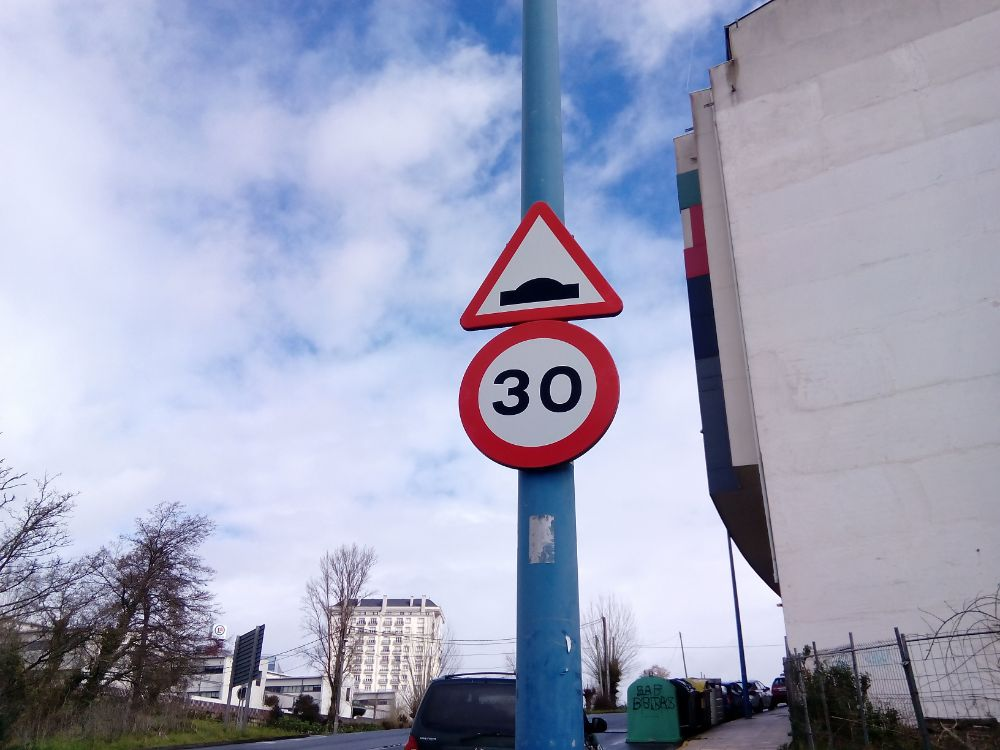
\includegraphics[height=4cm]{img/act0-1.jpg}
  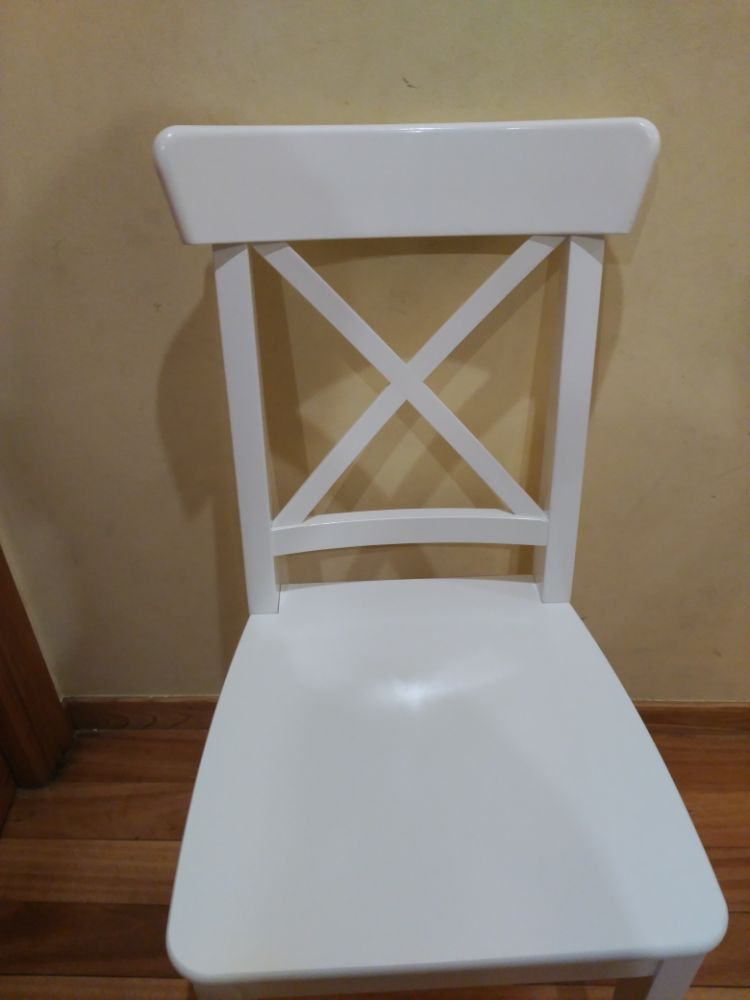
\includegraphics[height=4cm]{img/act0-2.jpg}
  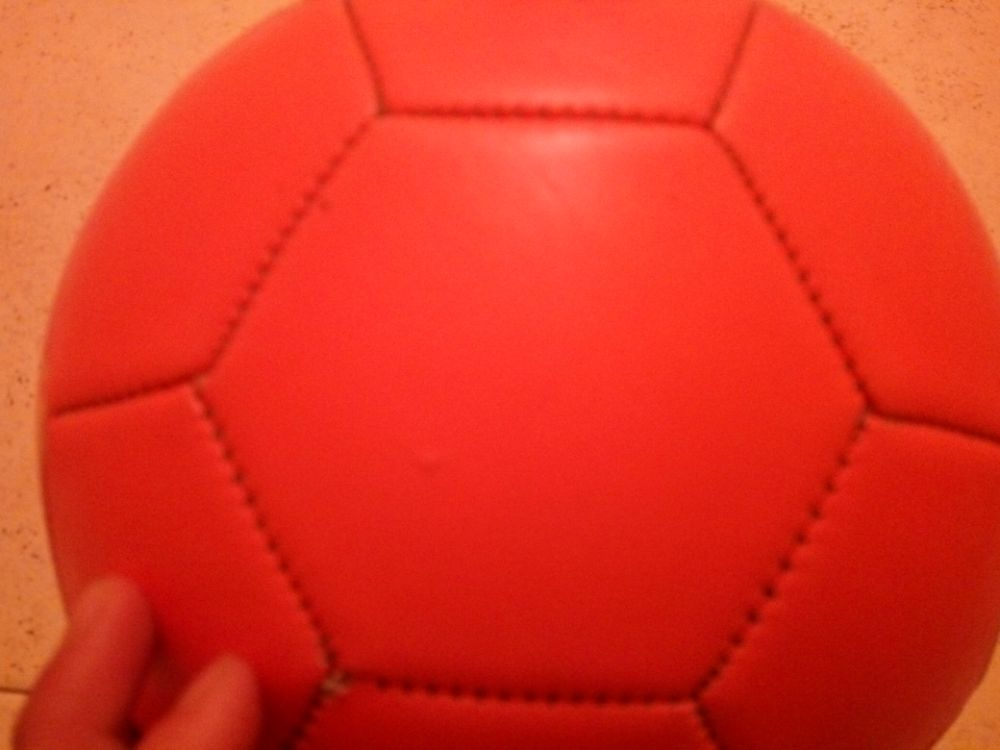
\includegraphics[height=4cm]{img/act0-3.jpg}
  \caption{Imaxes enviadas polos alumnos para a primeira actividade.}\label{fig:act0}
\end{figure}

Todas as fotos enviadas polo alumando serán subidas a web da materia. Na Figura~\ref{fig:act0} pódese ver algún exemplo do tipo de fotos que se buscan.

\subsubsection{Act. 1: Xeometría}
Como primeira activade do bloque de xeometría realizamos esta breve actividade introdutoria que pretende introducir ao alumnado no mundo da xeometría a par que se intenta habitualos nunha nova dinámica de clase na que se buscan a interacción docente-discente. Para introducilos no mundo da xeometría pedimos que definan coas súas palabras o que é a xeometría e a continuación mandarlles buscar por internet definicións de xeometría para que sexan lidas en voz alta. Para a realización desta actividade gastaremos sobre 10 minutos.

\subsubsection{Act.2: Puntos, liñas e posición relativa de liñas}\label{act2}
Durante esta actividade empezamos a explicar os elementos básicos de xeometría. Para facer isto comezamos preguntándolle aos alumnos e alumnas cal é para eles o elemento da xeometría máis simple que poden dicir. A raíz desta pregunta explicamos o concepto de punto. A raíz do punto explicamos que aliñando puntos obtemos unha recta. Explicase empregando un exemplo do programa Geogebra que a recta é infinita e que polo tanto non ten principio nin fin. A continuación expoñemos como se constrúe unha semirrecta, un segmento e detallamos a clasificación de rectas en función da súa posición relativa.

Para practicar a posición relativa das rectas realizamos unha actividade coas fotos de elementos xeométricos que enviaron na Actividade 0 (Sección~\ref{act0}). Durante esta actividade dividimos ha clase en grupos e cada grupo debe sinalar nas fotografías as rectas que sexan perpendiculares, secantes e paralelas. Para sinalar as rectas empregarase o programa de edición fotográfica, como pode ser GIMP.

\begin{figure}[h!]
  \centering
  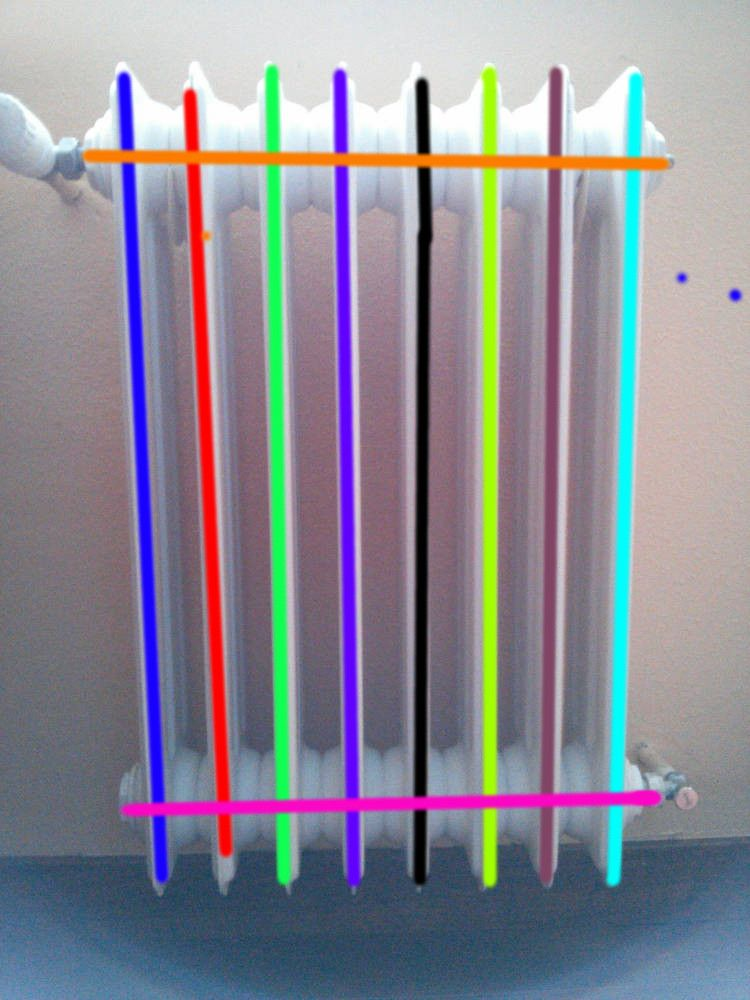
\includegraphics[height=4cm]{img/act1-img.jpg}
  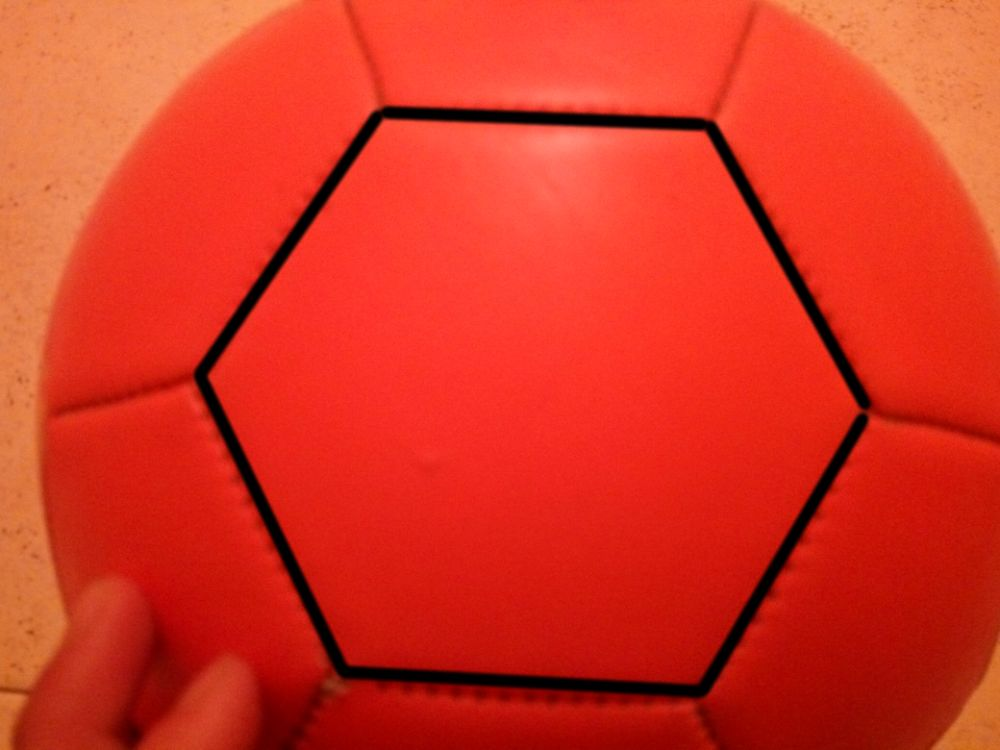
\includegraphics[height=4cm]{img/act1-img2.jpg}
  \caption{Marcado das imaxes con liñas paralelas, secantes e perpendiculares}\label{fig:act2}
\end{figure}

Despois de debuxar as rectas, os ficheiros son gardados e enviados por correo electrónico para ser proxectadas na clase. Cada grupo deberá explicar porque as rectas seleccionadoras teñen unha clasificación ou outra. Na Figura~\ref{fig:act2} pódense ver exemplos do que se pretende acadar. Dedicaremos a esta actividade aproximadamente 40 minutos.

\subsubsection{Act. 3: Ángulos e a súa clasificación}\label{act3}
Durante esta actividade explicaremos que é un ángulo así como a súa clasificación en función da súa amplitude e en función da súa posición relativa. Para practicar a clasificación de ángulos faremos un pequeno xogo onde as e os estudantes deberán por grupos clasificar diversos ángulos xerados aleatoriamente pola web \href{http://random.org}{Random.org}. Na Figura~\ref{fig:act5} pódese ver unha captura de pantalla dun ángulo xerado por esta web.

\begin{figure}[h!]
  \centering
  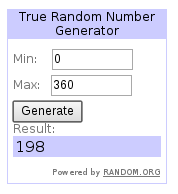
\includegraphics[height=5cm]{img/random.png}
  \caption{Captura de pantalla dun ángulo xerado por Random.org.}\label{fig:act5}
\end{figure}

\subsubsection{Act. 4: Sistema sexasesimal} %TODO
Explicamos o sistema sesaxesimal e como facer sumas e restas de grados expresados neste sistema. Baseamos a nosa explicación con unha comparación con algo que xa coñecen, a relación entre horas, minutos e segundos. Facemos varios exercicios propostos polo libro de texto sobre este tema.

\subsubsection{Act. 5: Mediatriz e bisectriz} %TODO
Explicamos os conceptos de mediatriz e de bisectriz e de como se trazan. Intentamos incidir nas propiedades que teñen a mediatriz e da bisectriz, e dicir, que os puntos destas dúas rectas equidistan dos extremos do segmento e dos lados do ángulo respectivamente. Estas propiedades serannos útiles máis tarde para explicar outros obxectos xeométricos como os puntos notables dos triángulos.

\subsubsection{Act. 6: Exame de xeometría básica}
Facemos un exame do explicado ata o momento que abrangue os conceptos de punto, rectas, planos, posición relativa de rectas, ángulos, clasificación de ángulos e posición relativa dos mesmos, sistema sesaxesimal, mediatrices e bisectrices. O exame que puxemos pódese ver no Apéndice~\ref{fich:ex1a}.

Intentando dar unha retroalimentación con respecto ao que o alumnado realizou neste exame o máis rápida posible corrixiremos os exercicios durante esa tarde e no día seguinte explicaremos todos os exercicios, os criterios de corrección e ensinámoslles ás alumnas e alumnos os exames corrixidos.

\subsubsection{Act. 7: Polígonos, triángulos e as súas clasificacións}\label{act7}
Expoñemos os conceptos de liña poligonal, de polígono e as clasificacións de polígonos en función dos seus ángulos e do número de lados. A continuación explicamos a clasificación dos triángulos en función dos seus ángulos e do número de lados iguais.

\begin{figure}[h!]
  \centering
  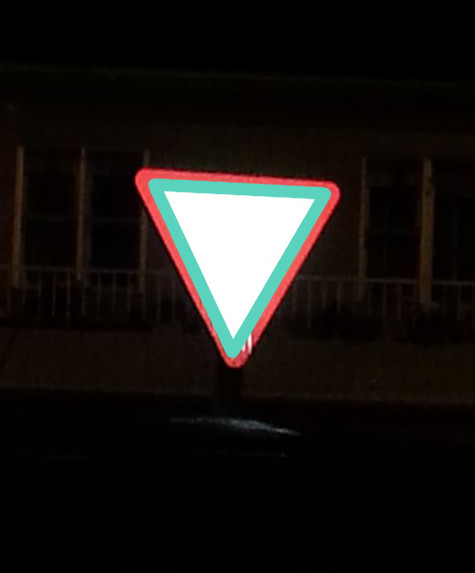
\includegraphics[height=5cm]{img/trian1.jpg}
  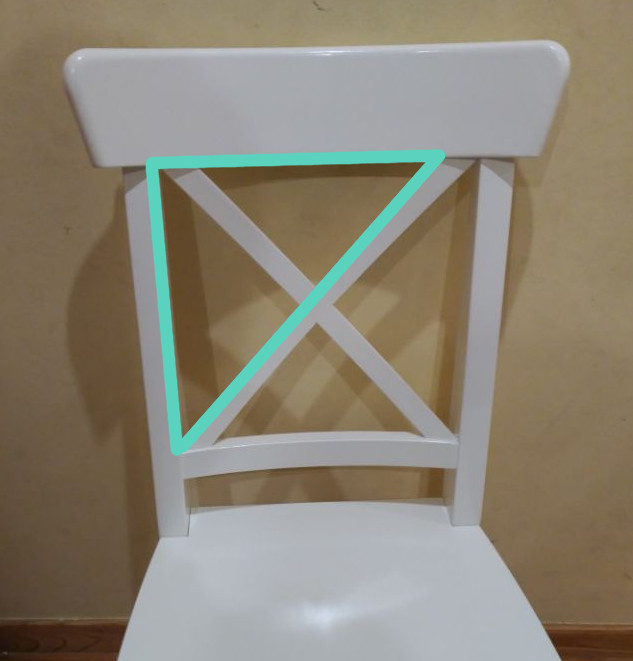
\includegraphics[height=5cm]{img/trian2.jpg}
  \caption{Exemplo de triángulo marcados sobre as fotografías}\label{fig:act7}
\end{figure}

Para practicar a clasificación dos triángulos realizamos un exercicio coas fotos que entregaron os alumnos durante a Actividade 0 (Sección~\ref{act0}). Para elo dividiremos a clase en grupos de 2 ou 3 persoas e cada grupo con un ordenador deberá buscar 4 triángulos diferentes nas fotos enviadas polos compañeiros. Da mesma forma que na segunda actividade, o alumnado deberá enviar as fotos editadas cos triángulos marcados ao ordenador do profesor no que se proxectarán. Cada grupo saíra e explicará a clasificación de cada un dos triángulos que marcou. Na Figura~\ref{fig:act7} pódense ver algúns exemplos das figuras que se pretenden acadar neste exercicio.

\subsubsection{Act. 8: Suma dos ángulos dun triángulo}\label{sec:sumang}
Nesta pequena actividade explicaremos e demostraremos de forma gráfica que a suma dos ángulos dun triángulo da sempre 180 grados. Para iso unha vez explicada esta propiedade na encerado, repartiremos triángulos feitos con goma-eva pero que, como se pode ver na Figura~\ref{fig:act11}, están partidos en tres fragmento de forma que se pode ver como poñendo os ángulos de forma consecutiva, obtense un ángulo llano.

\begin{figure}[h!]
  \centering
  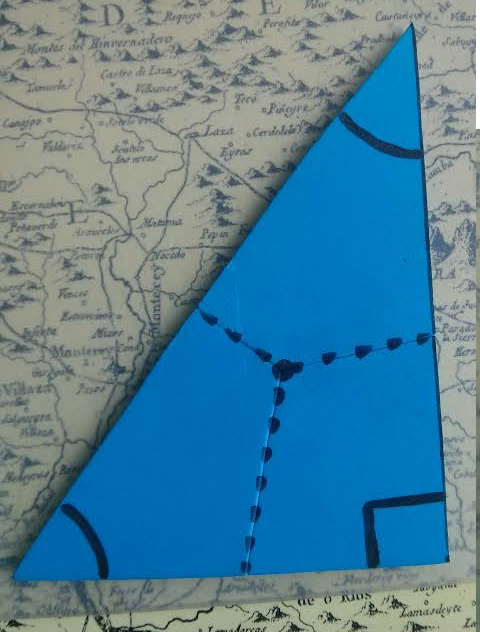
\includegraphics[height=5cm]{img/180grados-2.png}
  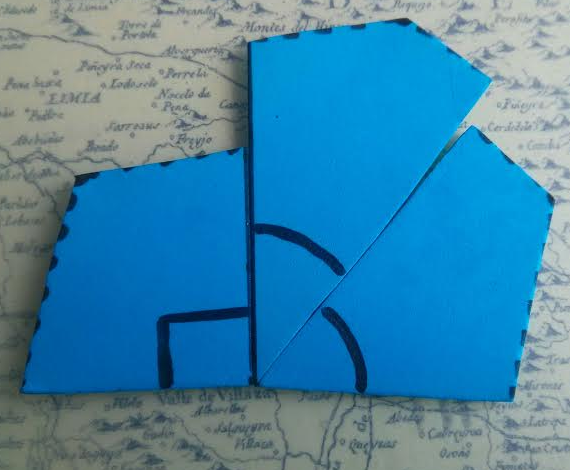
\includegraphics[height=5cm]{img/180grados-1.png}
  \caption{Figuras en goma-eva empregadas para ver a suma dos ángulos dun triángulo}\label{fig:act11}
\end{figure}

\subsubsection{Act. 9: Puntos e rectas notables do triángulo}\label{act9}
Explicamos os puntos e rectas notables recordamos primeiramente as definicións explicadas de mediatriz (como recta cuxos puntos equidistan dos extremos do segmento) e de bisectriz (como recta cuxos puntos equidistan dos lados do ángulo). Unha vez se repasaron estes conceptos, para explicar o circuncentro formulamos un problema no cal deberán buscar a posición ideal para colocar unha antena WiFi que abasteza ao instituto e a un hospital e centro comercial próximos. A formulación do problema acompoñámola coa imaxe que se pode ver na Figura~\ref{fig:act12-1}.

\begin{figure}[h!]
  \centering
  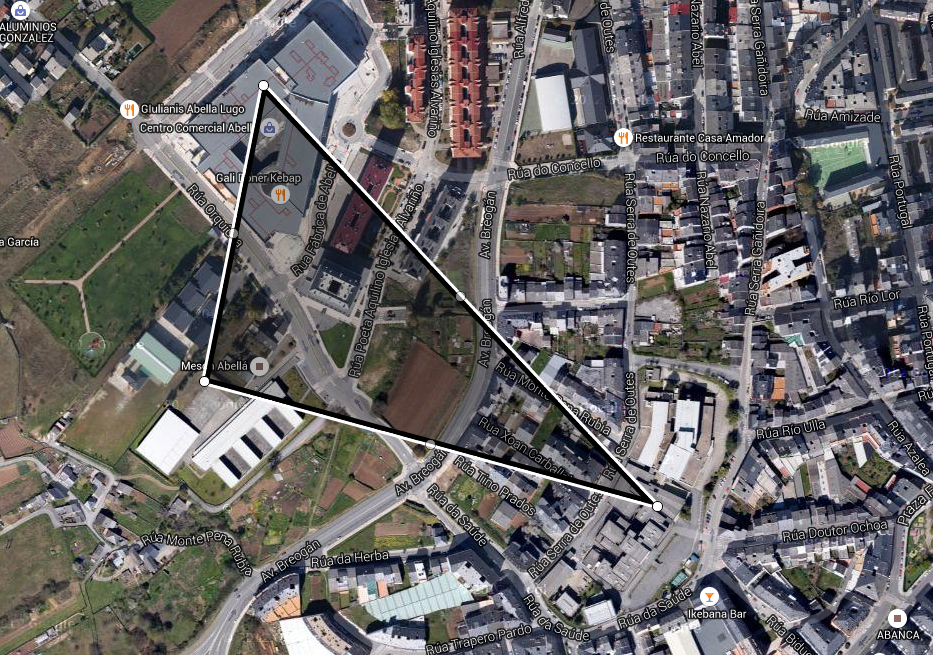
\includegraphics[height=5cm]{img/circuncentro.png}
  \caption{Imaxe empregada para explicar o circuncentro}\label{fig:act12-1}
\end{figure}

Pedimos que o alumnado formule como calcularían este punto e trázanse as solucións empregando o programa Geogebra. Explicamos porque as solucións propostas son ou non correctas e pedindo que expliquen porque a solución correcta consiste en trazar as mediatrices.

\begin{figure}[h!]
  \centering
  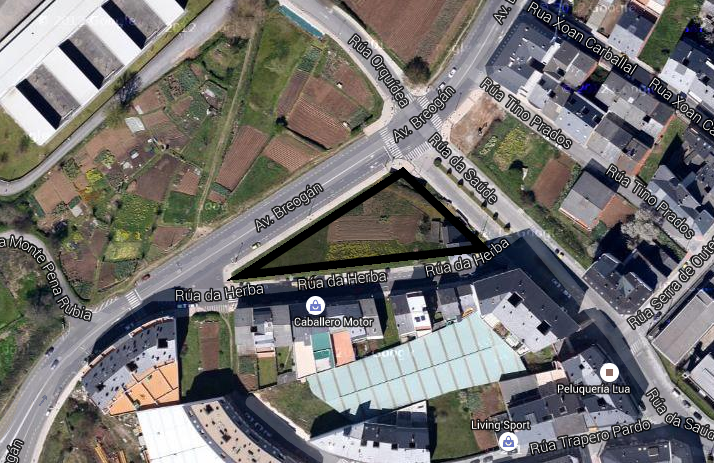
\includegraphics[height=5cm]{img/incentro.png}
  \caption{Imaxe empregada para explicar o incentro}\label{fig:act12-2}
\end{figure}

Para a explicación do dos demais puntos e rectas notables empregáronse métodos similares empregando a imaxe da Figura~\ref{fig:act12-2} para explicar o incentro e pedindo que dividan o triángulo en 6 partes de igual área no caso do baricentro.

\subsubsection{Act. 10: Teorema de Pitágoras}\label{act10}
Explicamos a denominación dos lados dun triángulo rectángulo e a relación entre a lonxitude destes. Relacionamos esta explicación coa area de cadrados con lados a hipotenusa e cada un dos catetos explicando que segundo o teorema cúmprese que a área do cadrado da hipotenusa é igual a suma das áreas dos cadrados dos dous catetos.

\begin{figure}[h!]
  \centering
  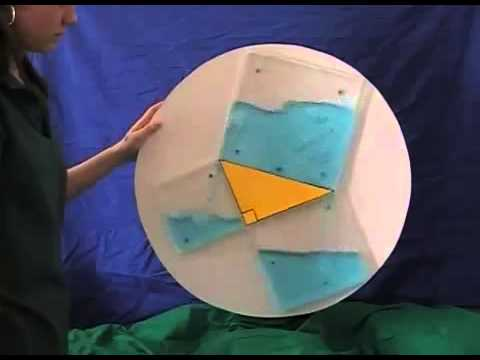
\includegraphics[height=7cm]{img/pitagoras.jpg}
  \caption{Captura dun dos vídeos proxectados con demostracións do Th. de Pitágoras}\label{fig:act10}
\end{figure}

Para reforzar o que explicamos na encerado proxectaremos varios fragmentos do documental \emph{Pitágoras: Mucha más que un teorema}\footnote{Este documental forma parte da serie Universo Matemático feito por RTVE que se pode ver completa en \href{http://www.rtve.es/television/la-aventura-del-saber/documentales/universo-matematico/}{rtve.es/television/la-aventura-del-saber/documentales/universo-matematico}.} relativos aos teorema. Ademais tamén se proxecta unha demostración feita con auga do teorema encontrada nun vídeo en YouTube\footnote{Pódese ver en \href{https://www.youtube.com/watch?v=1er3cHAWwIM}{youtube.com/watch?v=1er3cHAWwIM}.}. A captura da Figura~\ref{fig:act10} pertence a este último vídeo. Despois de ver estas demostracións, faremos exercicios propostos polo libro de texto.

\subsubsection{Act. 11: Clasificación cuadriláteros}\label{act11}
Explicamos a clasificación dos cuadriláteros e a continuación repetimos a mesma actividade que se realizou para practicar a clasificación dos triángulos.  Dividiremos a clase en grupos de 2 ou 3 persoas e cada grupo con un ordenador deberá buscar e marcar 4 cuadriláteros diferentes nas fotos enviadas durante a Actividade 0.
Os alumnos e alumnas enviaran as fotos modificadas ao ordenador do profesor para que estas sexan proxectadas e cada grupo lle poida explicar aos seus compañeiros a clasificación de cada un dos cuadriláteros que marcaron. Na Figura~\ref{fig:act11} pódese ver algún exemplo das figuras que pretendemos acadar.

\begin{figure}[h!]
  \centering
  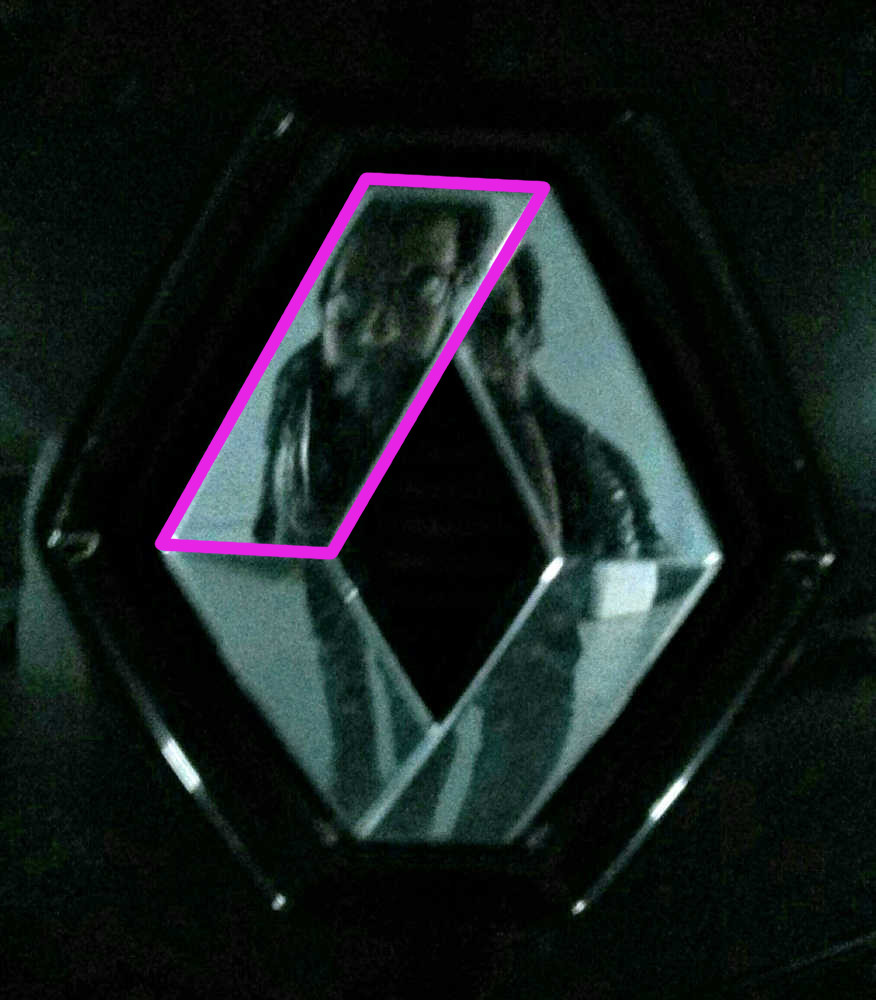
\includegraphics[height=5cm]{img/cuad1.jpg}
  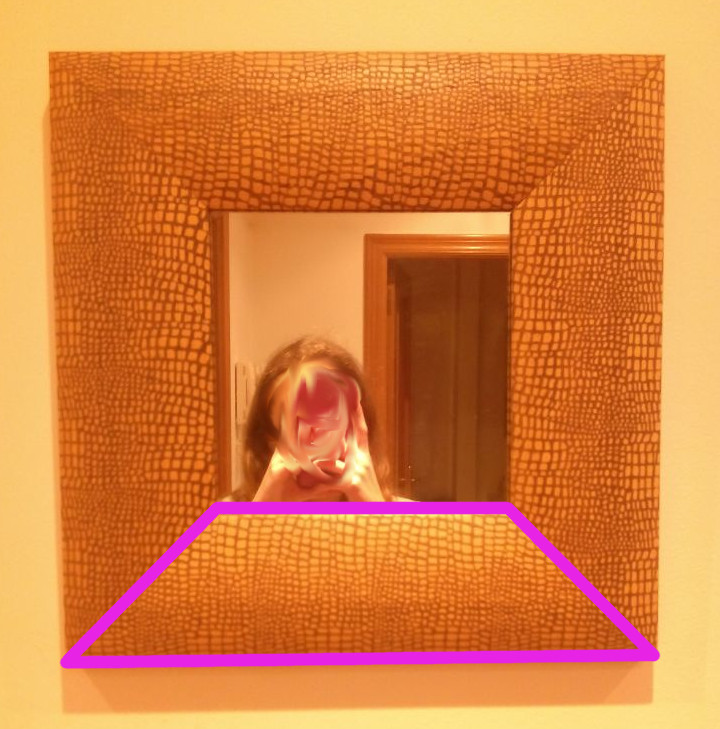
\includegraphics[height=5cm]{img/cuad2.jpg}
  \caption{Exemplo de cuadriláteros marcados sobre as fotografías}\label{fig:act11}
\end{figure}

\subsubsection{Act. 12: Elementos dos polígonos regulares. Circunferencia e círculo} %TODO
Durante esta actividade explicamos algún dos elementos dos polígonos regulares como o radio ou a apotema. Para explicar o concepto de circunferencia pedirémoslles ás alumnas e alumnos que formulen as súas propias definicións para ir corrixíndoas e terminar dando con unha correcta. Explicamos os elementos da circunferencia e por último o círculo e os seus elementos.

\subsubsection{Act. 13: Trivial de Polígonos}\label{act13}
Para practicar todos os conceptos traballados nas leccións anteriores trivial un trivial de 70 preguntas onde se repasan todos estes conceptos. Para facer isto empregamos a plataforma Socrative\footnote{Pódese acceder a ela en \href{http://www.socrative.com/}{socrative.com}.} que dispón dunha aplicativo móbil para a realización dos test así como a súa páxina web. Como se pode ver no Apéndice~\ref{fich:trivial}, as preguntas formuladas eran de varios tipos. Encontramos preguntas onde o alumnado debía seleccionar unha opción entre varias alternativas que lle eran dadas, preguntas onde debían dicir se un enunciado era correcto ou falso e preguntas onde eles mesmos debían escribir a resposta. Na Figura~\ref{fig:act13} pódese ver unha captura de unha posible pregunta que deberían responder as alumnas e alumnos.

\begin{figure}[h!]
  \centering
  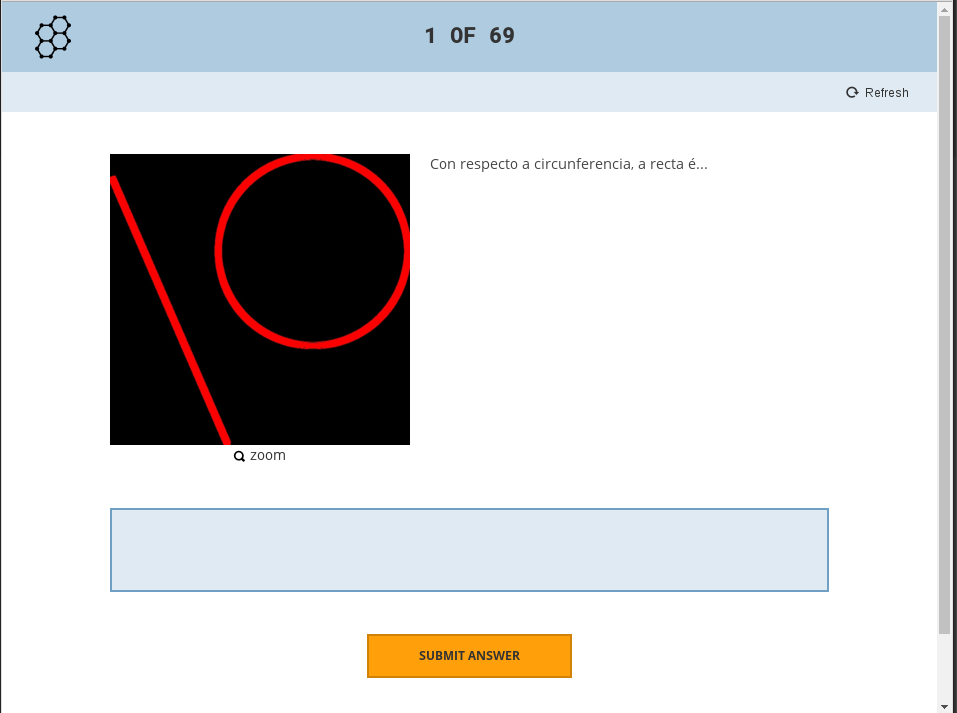
\includegraphics[width=0.8\textwidth]{img/socrative.png}
  \caption{Captura de pantalla dunha pregunta formulada na plataforma Socrative}\label{fig:act13}
\end{figure}

Para a realización do test dividiremos a clase en parellas e cada parella empregará un ordenador. Conectaranse á plataforma de Socrative e responderán a todas as preguntas durante a duración da clase. Durante a sesión seguinte a realización do trivial, analizaremos pregunta a pregunta cal é o resultado correcto e o porqué. Centrarémonos máis nos contidos que fallou a maior parte da clase.

\subsubsection{Act. 14: Exame polígonos}
Realizamos un exame dos contidos traballados anteriormente. O exame pode verse no Apéndice~\ref{fich:ex2}. Da mesma forma que fixemos no primeiro exame, corrixiremos os exames durante esa tarde para amosarllos ao día seguinte corrixidos e que reciban o \emph{feedback} o máis cedo posible.

%TODO: añadir actividade autoevaluación

\section{Valoración da aplicación da unidade e propostas de mellora}
%• Valoración da aplicación da unidade. Se por algunha circunstancia extrórdinaria non se puidese aplicar, a valoración referirase á idoneidade da unidade didáctica para o centro onde tiveron lugar as prácticas.
A maior parte das actividades desenvolvidas durante esta unidade didáctica foron postas en práctica durante o Practicum. Impartiuse en dous cursos de primeiro de ESO, un grupo grande de 18 estudantes e un agrupamento e so catro alumnos e alumnas. De seguido algunhas valoracións en canto a aplicación destas actividades.

Con respecto a \textbf{Actividade 0} (Sección~\ref{act0}), o resultado desta actividade foi peor do esperado. Por unha parte o alumnado expresou que non terminaba de entender o que se pedía polo que tivemos que explicar o que se pretendía lograr con esta actividade. Por outro lado, demostrouse que as alumnas e alumnos a pesar de teren case todos teléfono móbil e seren usuarios habituais de redes sociais como Instagram ou SnapChat, non tiñan un coñecemento sobre as tarefas ofimáticas máis básicas como pode ser a de enviar un correo electrónico. É subliñable neste sentido que un alumno confesou que este fora o primeiro correo electrónico que enviaba na súa vida. Ademais máis da metade dos alumnos non realizaron a actividade e non enviaron as fotografías. Por último, dentro das imaxes recibidas non había demasiada variedade e, por exemplo, para captar os triángulos, moitos alumnos recorrían a sinais de tráfico sendo isto un dos exemplos propostos durante a clase. Este feito provocou que fose necesario modificar algunha actividade na que era precisa unha certa variedade nas imaxes.

En canto aos resultados da \textbf{Actividade 2} (Sección~\ref{act2}), a parte realizada cos ordenadores foi de gran agrado para os alumnos segundo a enquisa de autoavaliación. Por outra parte isto pode ser debido simplemente a que tiñan que empregar os ordenadores non ao contido da actividade en si. Descubrimos que tamén había algún problema inicial por parte do alumnado para que empregasen o programa de edición proposto polo que sería interesante buscar unha alternativa que lles resultase máis sinxela. Ademais en canto ao tamaño dos equipos de traballo mencionar que os resultados foron moitos mellores no grupo reducido onde se traballou por parellas en lugar de grupos de tres a catro persoas. Esta última faceta foi resaltada pola propia titora que nos recomendou que traballasen por parellas.

Durante segunda parte da \textbf{Actividade 3} (Sección~\ref{act3}) xerouse unha certa dinámica competitiva entre un alumno e unha alumna do grupo grande se ben houbo outros alumnos que non participaron. En cambio no grupo reducido, o menor número de alumnos e alumnas permitiu que cada alumno clasificase varios ángulos diferentes e se practicasen máis estes conceptos.

As \textbf{Actividades 4 e 5} foron bastante aburridas e pouco interesantes para os alumnos polo que sería moi interesante buscar algunha alternativa que lles fose máis significativa.

En canto ao \textbf{exame} realizado dos conceptos básicos de xeometría, o exame realizado polo alumnado do grupo reducido foi diferente pois realizouse antes de explicar o concepto de mediatriz e bisectriz e os exercicios relacionados con este tema foron eliminados. Neste grupo tamén se detectou que parte do alumnado lle era moi complicado entender algún dos conceptos traballados cando non estaban dispostos por separado. A gráfica empregada no exame onde aparecen varias liñas paralelas, secantes e perpendiculares formando a súa vez ángulos diferentes, pareceulles moi difícil a pesar de tela utilizado con anterioridade nas explicacións.

Tivemos que modificar as \textbf{Actividades 7} (Sección~\ref{act7}) e \textbf{11} (Sección~\ref{act11}) debido a que nas fotos entregadas polo alumnado non había suficiente variedade. Como alternativa planteamos que en vez de buscar os polígonos nas fotos os debuxasen nunha folla en branco. Esta modificación causou que fose moito menos atractiva para o alumado. Unha mellor opción atopándose nesta situación sería procurar nós imaxes onde aparecesen máis variedade de polígonos para poder seguir empregando as imaxes.

Da \textbf{Actividade 9} (Sección~\ref{act9}) destacar que o alumnado participou activamente na busca de posibles solucións aos problemas plantexados e razoaron bastante adecuadamente os procedementos seguidos. Na \textbf{Actividade 10} (Sección~\ref{act10}) os alumnos quedaron moi impresionados con algunha das demostracións gráficas feitas nos vídeos proxectados.

En canto á \textbf{valoración global} feita polo alumnado a maioría valorou de forma positiva a nosa estadía no centro e destacaron como aspectos a mellorar, que explicase máis lento, que fixese máis exercicios e que mellorase a caligrafía. Por outro lado en conversacións informais cos estudantes, resaltaban que lles gustaría que as matemáticas fosen moito máis prácticas e comparábanas coa forma práctica coa que explicaba a bioloxía a súa profesora. A actividade que máis gustou a maioría de alumnos segundo a auto-avaliación foi o Trivial de Polígonos plantexado na Actividade 13 (Sección~\ref{act13}). Aínda que igual que pasou en actividades anteriores isto pode ser debido ao uso de ordenadores para realizala.

Como \textbf{reflexión global} sobre a posta en práctica desta proposta didáctica, dicir que quizais o fallo máis importante desta proposta didáctica sexa a pouca realización de exercicios similares aos do exame que se realizaron na aula. Sería moi interesante ver os resultados desta mesma proposta dedicando algunhas sesións a realización de exercicios. Neste sentido as críticas do alumnado son totalmente certas. Con respecto a velocidade de explicación e a caligrafía é dende logo un aspecto a corrixir na nosa práctica docente.

Con respecto as actividades propostas, pensamos que a maioría resultaron moi interesantes para o alumando e que lles acercaron a xeometría en particular e as matemáticas en xeral dunha forma diferente á que estaban acostumados.
